\chapter{Facility Layer \label{chap:facilitylayer}}
\begin{figure}[htbp]
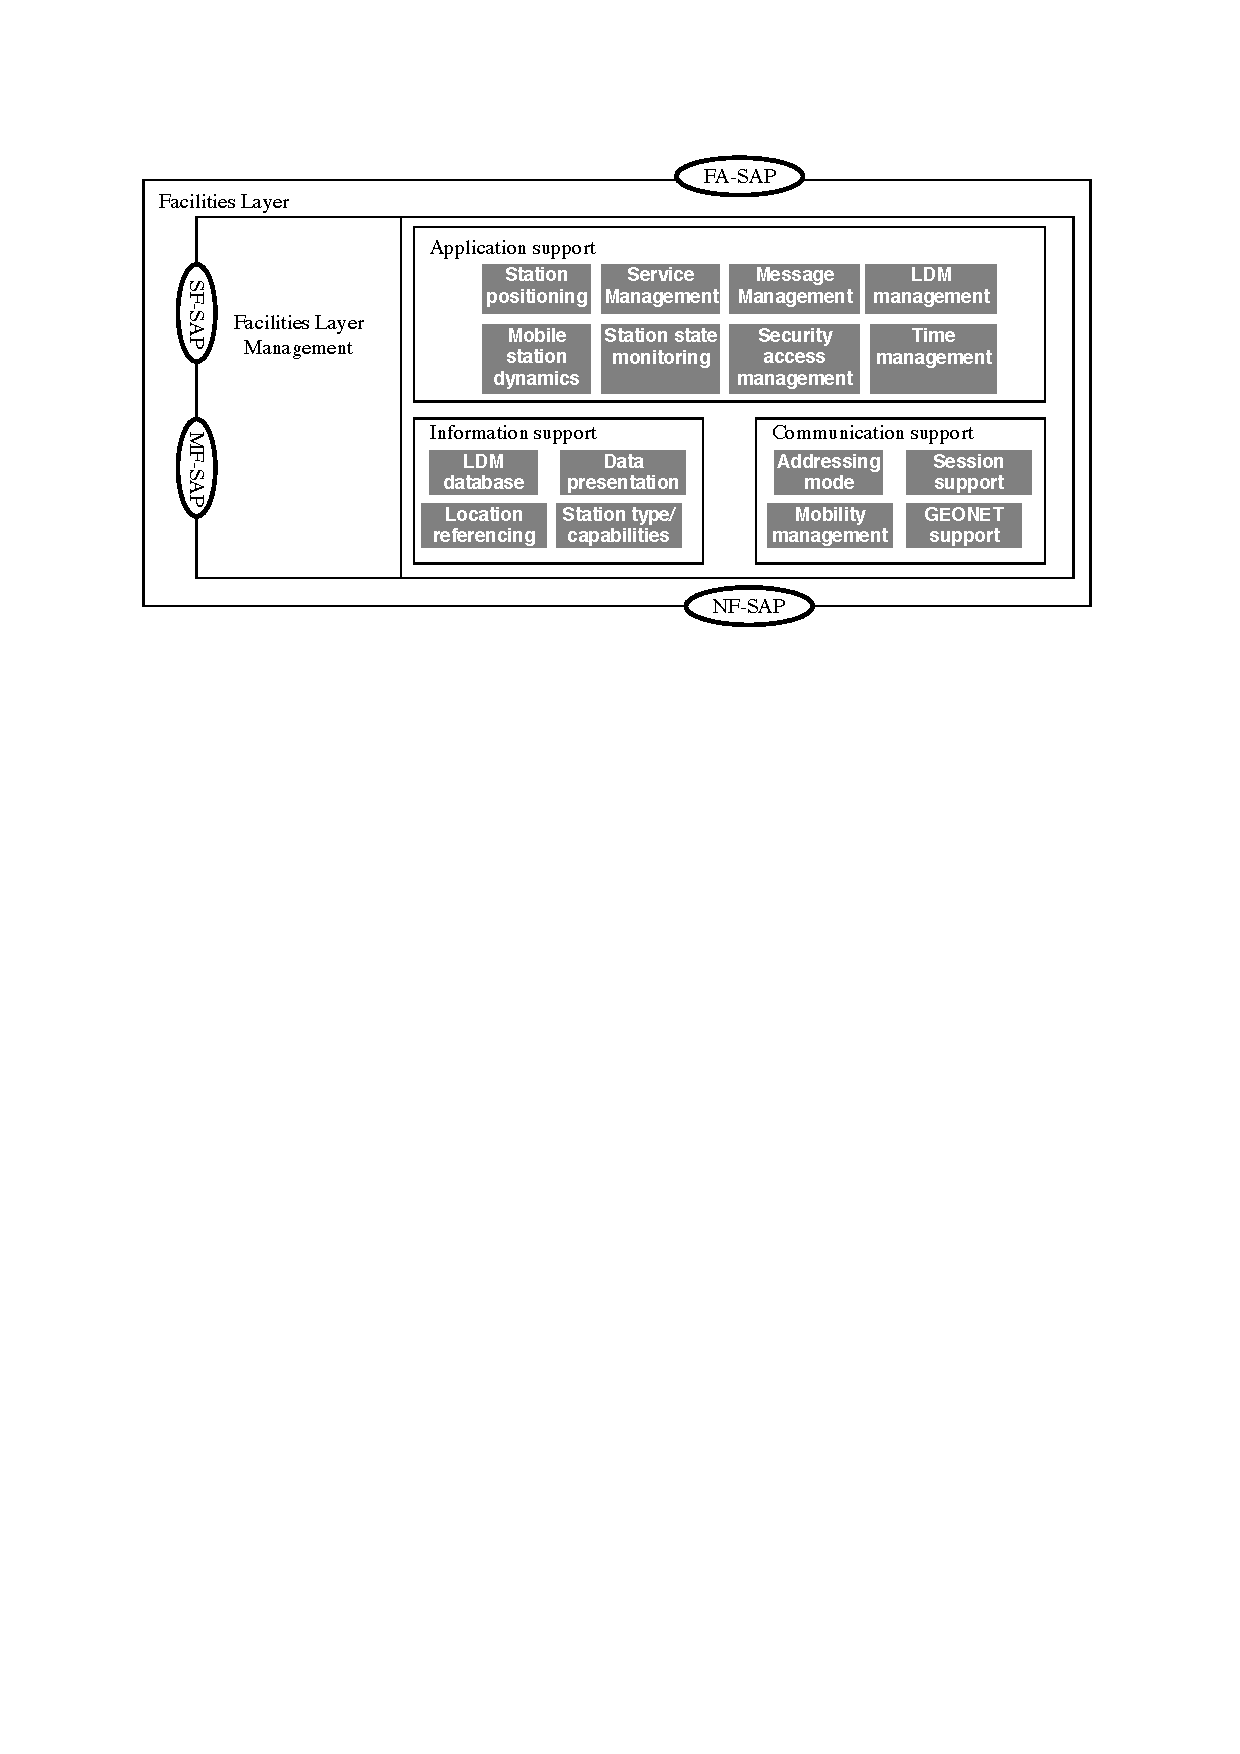
\includegraphics[width=0.99\textwidth]{content/images/04_facilitylayer/facility_layer_model.pdf}
\caption{Die Komponenten der \acl{C2C}}
\label{fig:komponentenfacility}
\end{figure}
Der Facility Layer liegt unterhalb des Applicationlayer und teilt sich in drei Hauptkomponenten auf. Er bietet verschiedene allgemeine Services an die von den Anwendungen des Application Layer verwendet werden können.

\subsection{Application Support}
Der Application Support stellt die Grundfunktionalität für die Anwendungen zur verfügung. Darunter fällt das station lifecycle management, das automatische erkennen von Services sowie das downloaden und initialisieren von neuen Services und noch weitere. Die einzelne Komponenten des Application Support, die auf der \autoref{fig:komponentenfacility} zu sehen sind, werden im folgenden genauer erläutert. 

\subsubsection{Station positioning}
Dieser teil des Application Support verarbeitet die Informationen die aus den verschiedenen Datensammler gewonnen werden wie aus GNSS oder aus Fahrzeugsensoren um die Position des Station zu gewinnen. 
Da diese Angaben sehr genau sein müssen werden die Daten in 3D Position gemessen (latitude, longitude, altitude). Dies können, durch beispielsweise GPS, in Echtzeit zur verfügung stehen. Da es jdeoch Sicherheitsbedingte Anwendungen gibt bei denen bereits über 0.5m Abweichung eine fatale Auswirkung haben kann, werden die Standortinformationen noch einmal über weitere Einheiten verbessert. Dazu gehören z.b. odometer oder gyroskop.

\subsubsection{Mobile station dynamic monitoring}

\subsubsection{Station state monitoring}

\subsubsection{Services management }

\subsubsection{LDM management }

\subsubsection{Messages management}

\subsubsection{Security access management}
\subsubsection{Time management}
\subsubsection{Time management}
\subsubsection{Time management}

\subsection{Information Support}
The information support covers the presentation layer of the OSI reference model and holds the role of
data management. In any ITS system, there will be an abundance of data sources, both mobile and static
ones. These data will mostly be location referenced, time specific and attached with life time value and
with accuracy and reliability parameters. Therefore, fusing data and keeping the information up to date is
one of the challenges of information support. Main entity that supports this is Local Dynamic
Map (LDM) that is able to take data both from different sources and from received ITS messages to build
a data model of the local environment. Furthermore, the information support takes on many functions of
the OSI Presentation Layer. 

\subsection{Communication Support}
The communication support, which includes the session layer of the OSI Reference model. It will
cooperate with the transport and network layer to achieve the various communication modes required by
the applications. 

\section{CAM\label{sec:cam}}

\section{DEN\label{sec:den}}


\section{SPaT\label{sec:spat}}

\section{TOPO\label{sec:topo}}
